\chapter{Environment on Mars}\label{ch:environmentOnMars}

Mars, also called the Red Planet, was named by the Romans after the god of war because of its red, blood-like color, see figure. 

\section{Terrain} 
The martian terrain contains certain features, the most notables of which are

\subsection{Tharsis and Elysium volcanic provinces,}
On the western hemisphere of Mars there is a huge volcano-tectonic known as Tharsis, which covers thousands kilometers in diameter and covers 25 \% of the planet\cite{surface}. %Being 7 to 10 kilometer higher than martian sea level which  is the highest in the solar system\cite{surface}.

\subsection{Large impact basins and Impact craters}
Impact craters are remnants of past collisions with certain types of asteroid on the surface of mars. The craters size can vary from small to very big such as Hellas basin which is 1800 km in diameter.

% The craters vary in size, the largest is named Hellas basin which is 1800 kilometer in diameter.

\subsection{Equatorial canyon system}
On the western hemisphere of Mars there is a large interconnected system of canyons. It extends eastwards for 4000 km and in some places it is as wide as 300 km and as deep as 10 km. These canyons are the result of tectonic movement.

\subsection{Chaotic terrain and outflow channels}
There exist certain filled up round hole places on the mars where the surface has collapsed, which are called chaotic terrain and seem to be the result of huge outflow of water or lava resulted from martian volcanic activity.

\subsection{Ice caps}
Seasonal Ice caps consist of carbon monoxide, water and dust, which covers both of Mars poles and can reach as high as 3 km in height and estimated to be as wide as 1000 km.

\subsection{Possible caves}
Observing from odyssey spacecraft, NASA scientists have identified seven possible caves. The entrance of these pits are 100 to 252 meters wide and they are believed to be around 70 to 96 meter in depth\cite{surface}\cite{guide}.

\subsection{Soil and water }
Mars surface is covered with rocks, sand and dust similar to some regions on earth, except that no organic material has yet been found on mars. The chemical composition of Mars soil can differ depending on where a sample has been taken, but the most known and symbolic element found is Iron in the form of rusting iron oxide, which gives the planet its famous red color. some of other chemical compounds that has been found on mars can be seen in the figure below.
\newline All evidence suggests that Mars used to have a watery past like that of earth, and water has been found in all three states: solid ice, gas and occasionally liquid in some specific areas\cite{liquid}.
more than five million cubic kilometer of water in the form of ice  has been identified close to  the surface of Mars\cite{water}.



\section{Climate of Mars}
The main composition of the martian atmosphere is carbon dioxide, and it has the surface pressure of 600 Pa where on earth, the atmospheric pressure on the surface is 101000 Pa.
\newline The surface of mars has a low thermal inertia, meaning that it heats up fast when under the sun light. At noon and near the equator, temperature reaches as high as 20$^{\circ}$C and at the poles it is around −153$^{\circ}$C. Thermal inertia changes in some areas on mars away from the poles, resulting in daily temperature swings and winds, which in return can pick up dust particles into the air and create clouds. Mars' atmosphere has a scale height of approximately 11 km\cite{climate}.


\newpage
\section{Force of gravity}
Gravitational acceleration of Mars is 3.711 m/s$^2$. The force of gravity upon a rover is calculated theoretically based on newton's second law of motion.
$$f=ma$$
$f$ being the downward force, $m$ mass and $a$ the acceleration.

\begin{figure}[h]
    \centering
    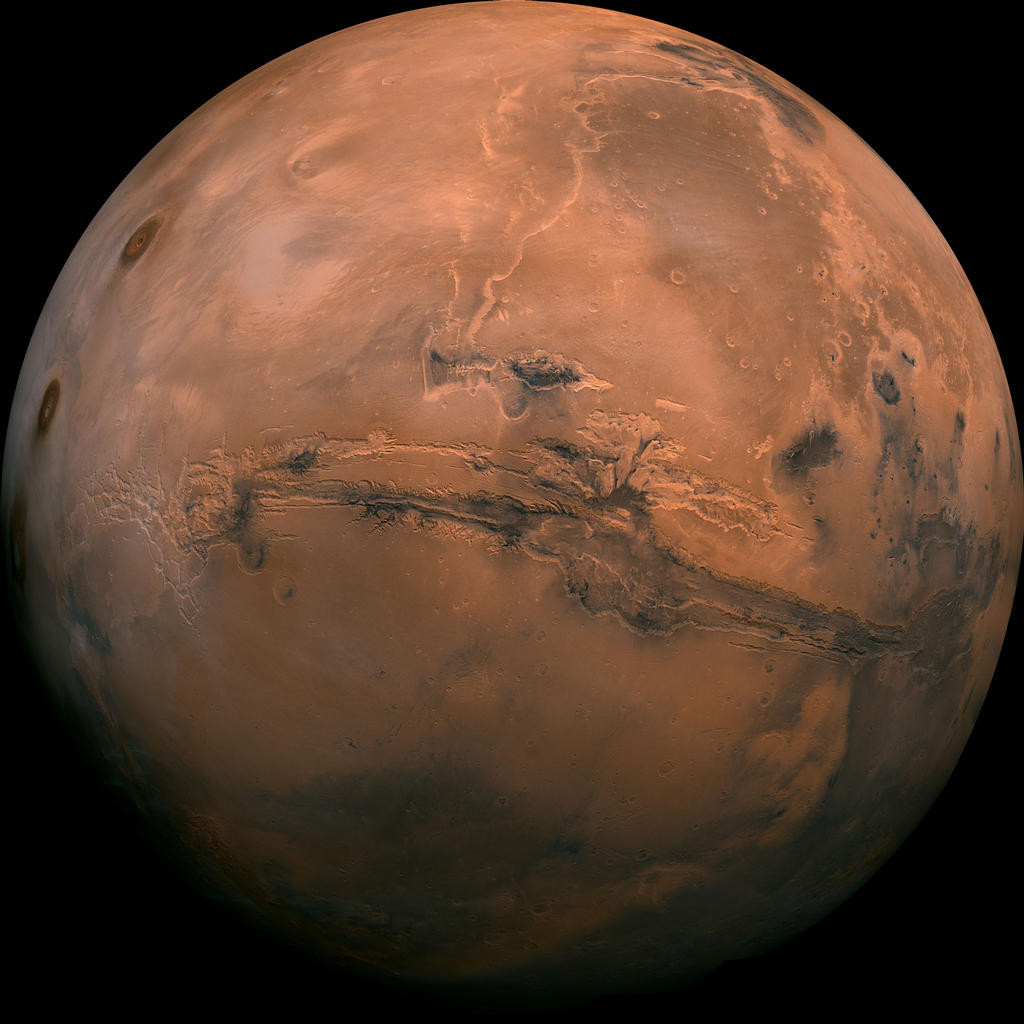
\includegraphics[width=.5\linewidth]{figures/marsImage01.jpg}
    \caption{Mars; also known as the Red Planet\cite{MarsPicture01}}
    \label{fig:marsPicture01}
\end{figure}


%As mentioned earlier, Mars has four seasons due to the tilt of its rotational axis just like Earth. Mars’ orbit is slightly elliptical which affects the length of its seasons and is about 1.5 times farther from the sun than Earth’s orbit therefore the seasons on Mars lasts about twice as long, see figure \ref{fig:marsSeasons} for a graphic illustration of the difference between Mars and Earth when it comes to seasons\cite{MarsBasicFacts}\cite{MarsOverview}\cite{gravity}\cite{MarsInDepth}.


%As seen on figure \ref{fig:marsSeasons}, the months on Mars are not only longer than the ones on Earth, but the seasons’ positions are different as well. When there is summer and winter on Earth, Mars experiences autumn and spring. This has something to do with how the planets tilt of its rotational axis to do.\todo{rewrite.. A bit messy} Both Earth and Mars have close to the same axial tilt, but the two planets do not point in the same direction in space. This is the reason to why Mars is about one season ahead compared to Earth\cite{MarsSeasons}
.
%Make this table more beautiful later on: https://da.sharelatex.com/learn/Tables
\begin{table} [h]
    \centering
    \begin{tabu} to 1\textwidth { | X[c] X[c] X[c] | }
     \hline
      & Earth & Mars \\ 
     %\hline
     %Average Distance from Sun & 150 million KM & 228.5 million KM \\  
     %\hline
     %Average Speed in Orbiting Sun & 29.7 KM/Sec & 23.3 KM/Sec \\
     %\hline
     %Diameter & 12,755.6 KM & 6,791.4 KM \\
     %\hline
     %Tilt of Axis & 23.5$^{\circ}$ & 25$^{\circ}$\\
     \hline
     Length of Year & 365.25 days & 687 Earth Days \\
     \hline
     Length of Day & 23 hours 56 minutes & 24 hours 37 minutes \\
     \hline
     Gravity & 2.66 times that of Mars & 0.375 times that of Earth \\
     \hline
     Temperature ranges from & -125$^{\circ}$C at the poles & +20$^{\circ}$C at equator \\
     \hline
     Atmosphere & Nitrogen, oxygen, & Mostly carbon dioxide, \\
      & argon, others & some water vapor \\
     %\hline
     %Number of moons & 1 & 2 \\
     \hline
    \end{tabu}
    \caption{Mars compared to Earth\cite{MarsVSEarth}}
    \label{tab:marsEarthFacts}
\end{table}


%The average temperature of Mars is 77$^{\circ}$ Celsius colder than Earth, with an average temperature of - 63$^{\circ}$ Celsius, see table \ref{tab:marsEarthFacts}.

As seen on figure \ref{fig:image003.jpg}, Earth and Mars are compared to each other as to the differences between the days in a year, gravity, sunlight and atmosphere. 

\begin{figure}[h]
    \centering
    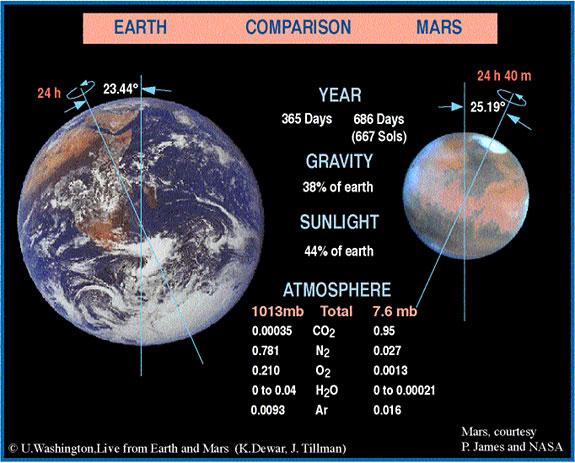
\includegraphics[width=.8\linewidth]{figures/image003.jpg}
    \caption{Earth and Mars comparison \cite{gravity}}
    \label{fig:image003.jpg} 
\end{figure}



%https://mars.nasa.gov/allaboutmars/facts/#?c=inspace&s=distance

%Write about Radiation, atmosphere and sunlight
%It is important to know: atmosphere and how much sunlight reaches Mars surface






%https://www.nature.com/articles/ngeo2412